%% Anona / drone_ws 正式技术报告
%% 版式：复用 arxiv-cjk-preprint 字体、段距、页眉页脚；不用「论文 picture」图题
%% 编译：latexmk -xelatex -shell-escape main-arxiv.tex
\documentclass[twocolumn]{article}

\usepackage{preprint}

%% 正文字号 12pt；行距 12/14
\makeatletter
\renewcommand{\normalsize}{%
  \@setfontsize\normalsize{12}{14}%
  \abovedisplayskip      8.5\p@ \@plus 2.5\p@ \@minus 5\p@
  \abovedisplayshortskip \z@ \@plus 3\p@
  \belowdisplayskip      \abovedisplayskip
  \belowdisplayshortskip 5\p@ \@plus 3\p@ \@minus 3\p@
}
\normalsize
\renewcommand{\small}{%
  \@setfontsize\small{10.5}{12.5}%
  \abovedisplayskip      7\p@ \@plus 2\p@ \@minus 4\p@
  \abovedisplayshortskip \z@  \@plus 2\p@
  \belowdisplayskip      \abovedisplayskip
  \belowdisplayshortskip 3.5\p@ \@plus 2\p@ \@minus 2\p@
}
\renewcommand{\footnotesize}{\@setfontsize\footnotesize{10}{12}}
\renewcommand{\scriptsize}{\@setfontsize\scriptsize{8.5}{10}}
\renewcommand{\tiny}{\@setfontsize\tiny{7}{8.5}}
\renewcommand{\large}{\@setfontsize\large{14}{16}}
\renewcommand{\Large}{\@setfontsize\Large{16}{19}}
\renewcommand{\LARGE}{\@setfontsize\LARGE{20}{24}}
\renewcommand{\huge}{\@setfontsize\huge{24}{28}}
\renewcommand{\Huge}{\@setfontsize\Huge{29}{34}}
\makeatother

\usepackage{fontspec}
\usepackage{xeCJK}
%% Linux：用 Liberation Serif 替代 Times New Roman
\setmainfont{Liberation Serif}
\setsansfont{DejaVu Sans}
\setCJKmainfont{Noto Serif CJK SC}[
  BoldFont = Noto Sans CJK SC,
  ItalicFont = Noto Serif CJK SC
]
\setCJKsansfont{Noto Sans CJK SC}

\usepackage{amsmath,amssymb}
\usepackage{xcolor}
\usepackage{graphicx}
\usepackage{caption}
\usepackage{enumitem}
\usepackage{booktabs}
\usepackage{microtype}
\usepackage{titlesec}
\usepackage{titling}
\usepackage{url}
\usepackage[colorlinks=true, linkcolor=black, urlcolor=blue!55!black, citecolor=black]{hyperref}

\graphicspath{{figures/}}
\renewcommand{\figurename}{图}
\renewcommand{\tablename}{表}
\DeclareCaptionLabelSeparator{cncolon}{：}
\captionsetup{labelsep=cncolon, font=small, labelfont=bf}
\renewcommand{\figureautorefname}{图}
\renewcommand{\tableautorefname}{表}

\usepackage{indentfirst}
\setlength{\parindent}{2em}
\setlength{\parskip}{5.5pt}

\makeatletter
\fancyhf{}
\lhead{\footnotesize\@title}
\rhead{\thepage}
\renewcommand{\section}{%
  \@startsection{section}{1}{\z@}%
                {-2.0ex \@plus -0.5ex \@minus -0.2ex}%
                { 1.5ex \@plus  0.3ex \@minus  0.2ex}%
                {\large\bfseries\raggedright}%
}
\renewcommand{\subsection}{%
  \@startsection{subsection}{2}{\z@}%
                {-1.8ex \@plus -0.5ex \@minus -0.2ex}%
                { 0.8ex \@plus  0.2ex}%
                {\normalsize\bfseries\raggedright}%
}
\makeatother

\titlespacing\section{0pt}{12pt plus 3pt minus 3pt}{1pt plus 1pt minus 1pt}
\titlespacing\subsection{0pt}{10pt plus 3pt minus 3pt}{1pt plus 1pt minus 1pt}
\titlespacing\subsubsection{0pt}{8pt plus 3pt minus 3pt}{1pt plus 1pt minus 1pt}

%% 章 = section；正文小节 = subsection
\makeatletter
\let\report@section\section
\let\report@subsection\subsection
\let\report@subsubsection\subsubsection
\newcommand{\chapter}{\report@section}
\renewcommand{\section}{\report@subsection}
\renewcommand{\subsection}{\report@subsubsection}
\newcommand{\chaptermark}[1]{}
\makeatother

\newcommand{\figwidth}{0.95\columnwidth}
\newcommand{\figmaxh}{0.42\textheight}
\raggedbottom
\newcommand{\ProjectFigure}[3]{%
  \par
  \noindent\begin{minipage}{\linewidth}
    \centering
    \includegraphics[width=\figwidth,height=\figmaxh,keepaspectratio]{#1}\par
    \vspace{0.15em}%
    \captionof{figure}{#2}%
    \label{#3}%
  \end{minipage}\par
  \vspace{0.85em}%
}
\newcommand{\ProjectTable}[1]{%
  \par\noindent\begin{minipage}{\linewidth}#1\end{minipage}\par\vspace{0.6em}%
}
\newcommand{\MapThumb}[1]{%
  \includegraphics[width=0.31\textwidth,height=0.18\textheight,keepaspectratio]{#1}%
}
%% 栏内并排：左场景 RViz，右评测曲线（禁止整页单图）
\newcommand{\ScenarioPair}[4]{%
  \begin{figure}[t]
    \centering
    \begin{minipage}[t]{0.48\linewidth}
      \centering
      \includegraphics[width=\linewidth,height=0.24\textheight,keepaspectratio]{#1}%
    \end{minipage}\hfill
    \begin{minipage}[t]{0.48\linewidth}
      \centering
      \includegraphics[width=\linewidth,height=0.24\textheight,keepaspectratio]{#2}%
    \end{minipage}
    \caption{#3}%
    \label{#4}%
  \end{figure}
}

\setlength{\droptitle}{-1.2em}
\title{基于 ROS~2 的模块化四旋翼仿真与多路径运动规划平台}
\author{Jungod\\[0.35em]
  {\normalsize 代码库 \texttt{drone\_ws}（工程名 Anona）}}
\date{}

\begin{document}

%% ========== 第 1 页：单栏 标题 / 作者 / 摘要 / 关键词 ==========
\onecolumn
\maketitle
\thispagestyle{empty}

\begin{abstract}
\noindent
四旋翼自主飞行软件常把刚体动力学、底层控制与运动规划捆在同一仓库树中。更换规划后端时，执行链路与评测脚本往往一并改动，不同算法难以在同一执行条件下公平对照。针对这一问题，本文实现并整理一套运行于 Ubuntu~22.04 与 ROS~2 Humble 的模块化四旋翼仿真平台（工程仓库名 Anona，代码库 \texttt{drone\_ws}）。平台将动力学与控制层（plant，即自研 X 布局刚体动力学、级联 PID 与混控）固定下来，以统一话题契约接入 Path~A--H 共八类规划后端，覆盖经典栅格搜索、反应式直方图、无 ESDF 局部重规划、MINCO/GCOPTER 与 Hermite 轨迹优化、FUEL 风格探索任务模式，以及极坐标 DrQ-SAC 学习策略。障碍地图全部为过程生成点云：既包括 EGO 谱系的 random\_forest / mockamap 官方资源，也包括自研 \texttt{drone\_map} 的密集场、开阔场与窄通道等，并由 \texttt{map\_adapter} 统一到双话题与元数据接口。

相对导师指定的 \texttt{pengyu\_sim} 与 MARSIM，本系统仅在概念上对照 RPM 到 wrench 分配、电机不对称滞后与仿真组织方式，动力学与控制器在 ROS~2 中独立实现，不执行、不包装其源码；官方规划器以 vendor 或桥接接入，剥离 SO3 / fake\_drone 等原仓库自带执行体，使对照落在规划算法而非各异的假飞机模型上。六项一键验收场景全部通过；七规划器$\times$两地图（官方森林与密集场）正方形任务在 staged 角点驻留规则下呈现显著差异。Path~H 在 dense\_field 对照中未能以策略本体完成成功判定（失败；安全监督 FALLBACK 不得记为纯 SAC 通过），单机循环演示取自随机森林而非密集场。正文给出动力学与控制全公式、地图目录、Path~A--H 模块对照表与统一接入说明、六项验收配对分析，以及可核验的开源关系专章，并讨论局限与后续工作。
\end{abstract}

\vspace{0.6em}
\noindent\textbf{关键词：}ROS~2；四旋翼动力学；级联控制；运动规划；仿真地图；开源对照；避障；仿真评测

\clearpage
%% ========== 第 2 页起：单栏目录 ==========
\tableofcontents
\clearpage

%% ========== 目录后：双栏正文 ==========
\twocolumn
\pagestyle{fancy}

%% 正文。术语：plant → 动力学与控制层（禁止“植物层”）。
%% 顺序：引言 → 架构 → 动力学/控制 → 实验 → 地图 → 单机飞行规划 → 多机飞行规划 → 控制台 → 开源 → 反思 → 感想
%% 配套测试报告与 AI 说明见仓库 report/appendix/（不编入 PDF）
\chapter{引言与项目目标}

四旋翼自主飞行软件常把刚体动力学、底层控制与运动规划捆在同一仓库树里。换规划后端时，执行链路和评测脚本也常一起改，算法对照就失去可比性。本报告所述仿真系统（工程名 Anona，代码库 \texttt{drone\_ws}）就是冲着这件事来的：在 Ubuntu~22.04 与 ROS~2 Humble 上固定动力学与控制层（plant：自研刚体动力学、级联 PID 与 X 型混控），用稳定话题契约接入 Path~A--H，再用同一套启动、地图与评测脚本做验收和批量对照。

相对任务参考的 \texttt{pengyu\_sim} 与 MARSIM，本系统按独立 ROS~2 工程来写：动力学与混控方程自行推导编码，运行时不执行、不包装对方动力学源码。规划侧经统一话题契约驱动同一控制器（见表~\ref{tab:contract}），而不是在第三方 SO3、MAVROS 或 fake\_drone 上做薄封装。EGO-Planner、GCOPTER、MIGHTY、Fast-Planner 等以 vendor 或桥接接入，使对照矩阵里积分频率、控制频率和安全判据保持一致。

\chapter{系统架构与模块化}

本系统按运维、规划、世界与动力学控制四层拆开，如图~\ref{fig:arch}。运维层负责一键 launch、浏览器/原生任务控制台与批量评测；规划层注册 Path~A--H（单机）；世界层由 \texttt{drone\_map} 或官方地图生成器出障碍点云，经 \texttt{map\_adapter} 统一话题；动力学与控制层由 \texttt{drone\_dynamics} 与 \texttt{drone\_controller} 固定。后文按单机飞行规划、多机飞行规划与任务控制台展开。

\ProjectFigure{architecture.png}{分层架构：运维、规划、世界与动力学控制层}{fig:arch}

模块化主要靠几条硬约束。动力学与控制层的话题和消息类型不随规划器改名：控制器始终订阅里程计与目标或轨迹指令，发布电机转速。地图差异多半只在点云话题名，适配后同时保留 \texttt{/map/obstacles} 与官方常用名。公平对照只收 weak / strong 后端（A/B/C/E/G/H）；探索模式 D 与谱系可选 F 不进主矩阵。统一数据流见图~\ref{fig:topics}。

\ProjectFigure{topic_dataflow.png}{单机统一话题契约与状态反馈}{fig:topics}

稳定契约见表~\ref{tab:contract}。目标可由 RViz“2D Goal Pose”或任务脚本发到 \texttt{/drone/goal}；规划路径用黄色 \texttt{/planner/trajectory} 显示，飞过轨迹为蓝色 \texttt{/drone/path}。RViz 用来看机体、障碍云和黄蓝轨迹，实验截图也来自同一布局（见图~\ref{fig:rviz}）。

%% 表1 | 图3：tabular* 满宽两列 + \vspace{0pt} 顶对齐（列内禁用 \\，改用 \par）
\par\medskip
\noindent
\refstepcounter{table}\label{tab:contract}%
\refstepcounter{figure}\label{fig:rviz}%
\begin{tabular*}{\linewidth}{@{\extracolsep{\fill}}p{0.48\linewidth}p{0.48\linewidth}@{}}
\vspace{0pt}\centering\normalsize
\setlength{\tabcolsep}{4pt}%
\begin{tabular}{@{}cll@{}}
\toprule
方向 & 话题 & 类型/说明 \\
\midrule
入 & \texttt{/drone/odom} & \texttt{Odometry} \\
入 & \texttt{/drone/goal} & \texttt{PoseStamped} \\
入 & 障碍云 & \texttt{PointCloud2} \\
出 & \texttt{/planner/local\_goal} & 滚动局部目标 \\
出 & \texttt{/planner/trajectory\_cmd} & $p,v,a,$ yaw \\
出 & \texttt{/planner/trajectory} & RViz 路径 \\
\bottomrule
\end{tabular}\par\vspace{0.5em}%
{\small\bfseries 表~\thetable：}{\small 规划器与动力学控制层的稳定话题契约}%
&
\vspace{0pt}\centering
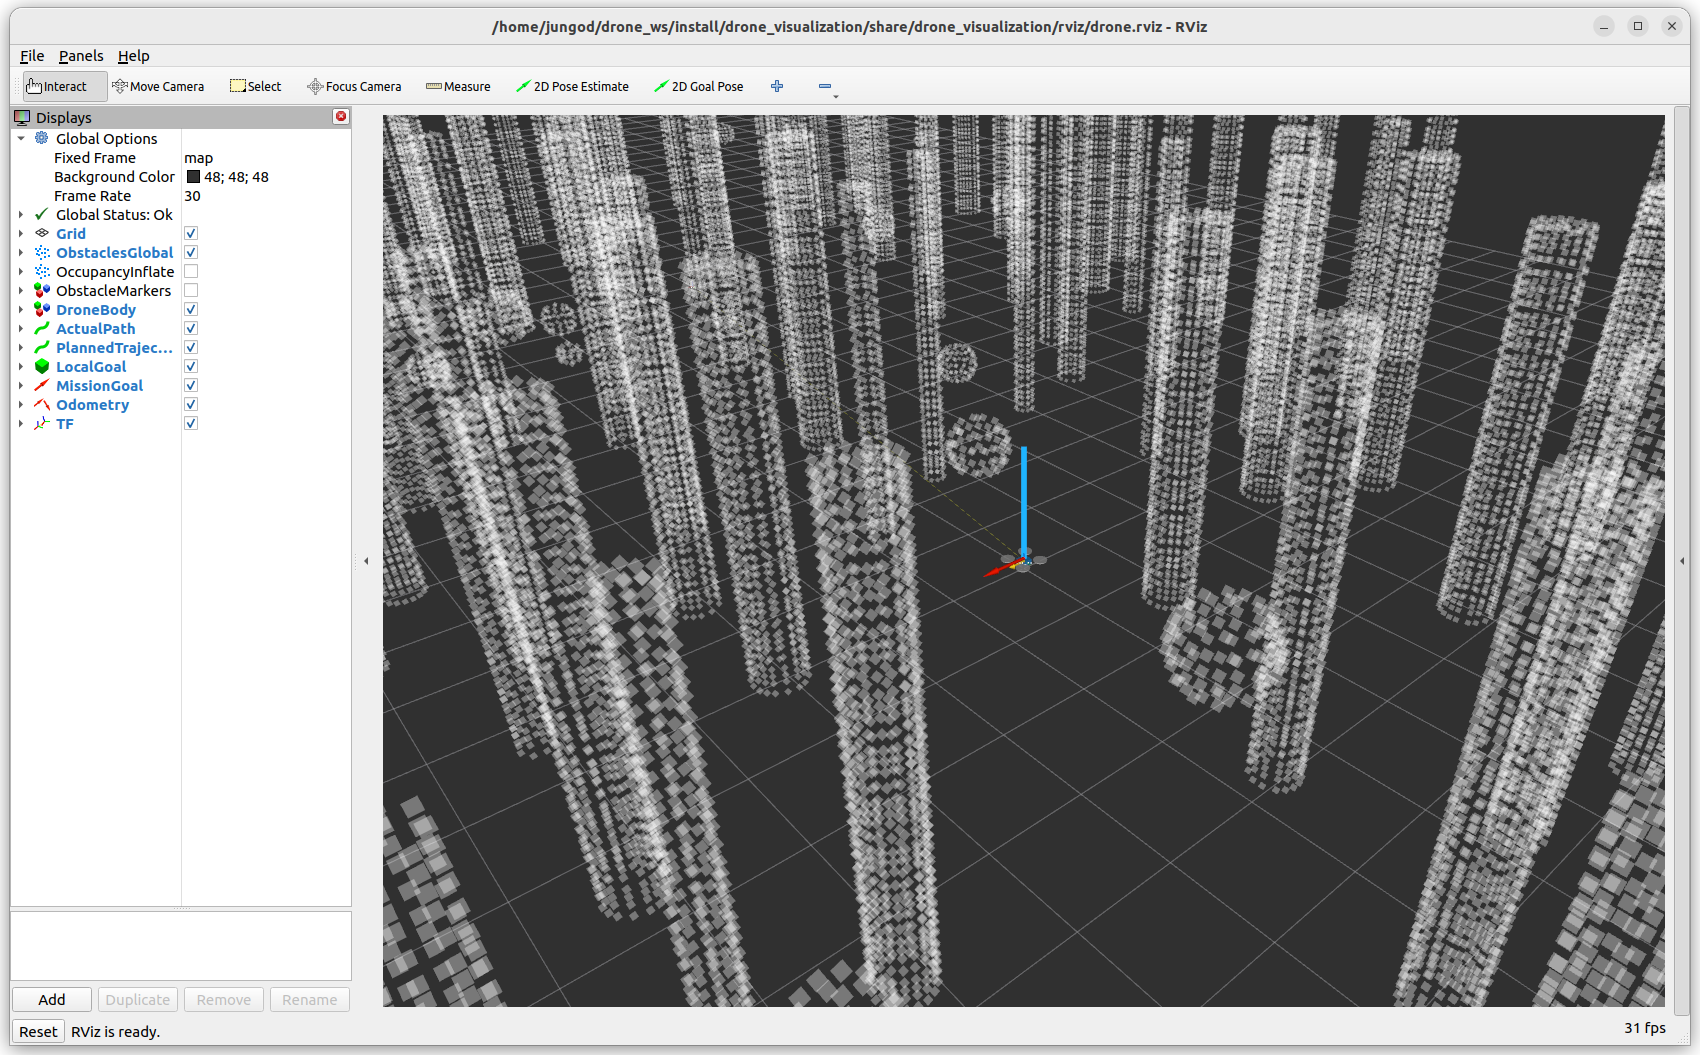
\includegraphics[width=\linewidth,height=0.22\textheight,keepaspectratio]{rviz_overview.png}\par\vspace{0.5em}%
{\small\bfseries 图~\thefigure：}{\small RViz 总览：机体、障碍、规划黄线与飞过蓝线}%
\end{tabular*}%
\par\medskip

\chapter{动力学与控制器}

\section{刚体状态与电机动力学}

状态取地图系 ENU 位置 $p\in\mathbb{R}^3$、速度 $v$、机体系到地图系姿态四元数 $q$、机体系角速度 $\omega$，以及四路电机角速度 $\omega_i$（内部为 rad/s；话题使用 RPM）。默认质量 $m=1\,\mathrm{kg}$，重力 $g=9.81\,\mathrm{m/s^2}$，臂长 $L=0.18\,\mathrm{m}$，惯量对角元 $I_{xx}=I_{yy}=0.01$、$I_{zz}=0.02$。推力与反扭矩系数分别为 $k_F=3\times10^{-5}$、$k_M=5\times10^{-7}$。

电机指令经一阶滞后跟踪，并允许升速/降速不对称时间常数 $\tau_{\mathrm{up}}$、$\tau_{\mathrm{down}}$（概念上对照 pengyu\_sim，实现为自研代码）：
\begin{equation}
  \dot{\omega}_i = \frac{\omega_i^{\mathrm{cmd}}-\omega_i}{\tau_i},\qquad
  \tau_i=
  \begin{cases}
  \tau_{\mathrm{up}}, & \omega_i^{\mathrm{cmd}}\ge\omega_i,\\
  \tau_{\mathrm{down}}, & \text{otherwise.}
  \end{cases}
\end{equation}
其中 $\omega_i^{\mathrm{cmd}}$ 由 RPM 指令换算并限制在 $[\omega_{\min},\omega_{\max}]$。

\section{分配矩阵与刚体方程}

X 布局电机顺序为前左(0,CCW)、前右(1,CW)、后右(2,CCW)、后左(3,CW)，杠杆臂 $l=L/\sqrt{2}$。令 $\Omega=(\omega_0^2,\omega_1^2,\omega_2^2,\omega_3^2)^\top$，则合推力与机体力矩
\begin{equation}
  \begin{bmatrix} T\\ \tau_x\\ \tau_y\\ \tau_z \end{bmatrix}
  = A\,\Omega,
  \quad
  A=
  \begin{bmatrix}
  k_F & k_F & k_F & k_F \\
  k_F l & -k_F l & -k_F l & k_F l \\
  -k_F l & -k_F l & k_F l & k_F l \\
  k_M & -k_M & k_M & -k_M
  \end{bmatrix}.
\end{equation}
平动与转动（可选风扰 $F_{\mathrm{ext}}$）为
\begin{align}
  m\dot{v} &= R(q)\,(0,0,T)^\top + (0,0,-mg)^\top + F_{\mathrm{ext}}, \\
  I\dot{\omega} &= \tau - \omega\times(I\omega),
\end{align}
其中 $R(q)$ 为姿态旋转矩阵。位置欧拉积分 $p\leftarrow p+v\Delta t$；姿态按 $\dot{q}=\tfrac12 q\otimes(0,\omega)$ 积分并每步归一化。地面采用单边约束与水平摩擦阻尼。积分 500\,Hz，状态与 IMU 发布 100\,Hz。运行日志标明动力学为自研，非 MARSIM / EGO 自带仿真器。

\section{级联 PID 与混控}

控制器与动力学共用同一分配矩阵。外环由位置误差生成期望速度并限幅，再经 PD/I（仅在近悬停 settling 时积分）与可选常值扰动观测得到期望加速度；由加速度构造倾转受限的推力方向与偏航，内环对姿态与角速度做 PD，得到机体力矩。混控求解
\begin{equation}
  \Omega = A^{-1}(T,\tau_x,\tau_y,\tau_z)^\top,
\end{equation}
再开方并换算为 RPM，施加斜率限制后发布至 \texttt{/drone/motor\_rpm\_cmd}。控制环 100\,Hz。追踪规划器滚动目标时关闭积分与扰动观测，以免把机体推入障碍。

\chapter{实验}

\section{六项验收场景}

按任务要求设悬停、单目标、多航点、静态避障、窄通道绕行与稳定性（误差/RPM 等曲线）六类场景。一键 launch 加 \texttt{scripts/run\_acceptance.py} 自动评测；六项全部通过（6/6 PASS），摘要见表~\ref{tab:accept}。悬停与点到点要求末段位置误差到 $0.3\,\mathrm{m}$ 以内；避障要求相对障碍云的最小间隙大于设定安全距离。每项说明后跟栏内配图：左 RViz，右评测曲线。

\ProjectTable{%
\captionof{table}{六项验收场景结果摘要}\label{tab:accept}
\centering
%% 铺满栏宽且不缩放字号（与正文 \normalsize 一致）
\normalsize
\setlength{\tabcolsep}{0pt}%
\begin{tabular*}{\linewidth}{@{\extracolsep{\fill}}cccc@{}}
\toprule
\# & 场景 & 关键指标 & 结果 \\
\midrule
1 & 悬停 & 终误 $0.0001\,\mathrm{m}$ & PASS \\
2 & 单目标 & 终误 $0.0013\,\mathrm{m}$ & PASS \\
3 & 多航点正方形 & 航点 $5/5$，终误 $0.0003\,\mathrm{m}$ & PASS \\
4 & 静态避障 & 最小障距 $0.313\,\mathrm{m}$，wp $8/8$ & PASS \\
5 & 窄通道 & 最小障距 $0.987\,\mathrm{m}$，终误 $0.0003\,\mathrm{m}$ & PASS \\
6 & 稳定性 & 终误 $0.0433\,\mathrm{m}$ & PASS \\
\bottomrule
\end{tabular*}}

\subsection{场景1：悬停}

\texttt{hover.launch.py}：开阔稀疏图，约 3\,s 后发布目标 $(0,0,1.5)$。机体从地面附近爬升并悬停；末段均值误差 $0.0006\,\mathrm{m}$，最终 $0.0001\,\mathrm{m}$，远低于 $0.3\,\mathrm{m}$ 阈值。图~\ref{fig:sc01} 左是悬停位姿与轨迹，右是位置误差与 RPM 曲线——开环无规划时，动力学与控制层闭环能站住。

\ScenarioPair{sc01_rviz.png}{sc01_eval.png}{场景1 悬停：RViz（左）与评测曲线（右）}{fig:sc01}

\subsection{场景2：单目标}

\texttt{single\_goal.launch.py}：目标 $(2,1,1.5)$。最终误差 $0.0013\,\mathrm{m}$，最大约 $0.11\,\mathrm{m}$（起飞过渡），末段能稳住。图~\ref{fig:sc02} 里机体直线接近目标后误差回落，点到点跟踪与限幅可用。

\ScenarioPair{sc02_rviz.png}{sc02_eval.png}{场景2 单目标：RViz（左）与评测曲线（右）}{fig:sc02}

\subsection{场景3：多航点正方形}

\texttt{multi\_goal.launch.py}：原点起步的 $2\,\mathrm{m}\times2\,\mathrm{m}$ 闭合正方形，到点且低速后切下一航点，共 $5/5$ 航点（含回起点），最终误差 $0.0003\,\mathrm{m}$。图~\ref{fig:sc03} 左折线贴合正方形，右图误差在换点时尖峰后很快落下，航点状态机和控制器衔接正常。

\ScenarioPair{sc03_rviz.png}{sc03_eval.png}{场景3 多航点：RViz（左）与评测曲线（右）}{fig:sc03}

\subsection{场景4：静态避障}

\texttt{avoidance.launch.py}：Path~B（EGO）+ \texttt{official\_forest}；任务第一圈矩形、第二圈漏斗航线，强制绕障。评测图里 XY 呈多圈闭合折线，是航点序列本身，不是乱飞；相对瞬时目标的位置误差偏大也属预期，不以全程均值误差作通过条件。规划器报过 success，循环航点 $8/8$ 都走到；相对障碍云最小间隙 $0.313\,\mathrm{m}$（安全阈 $0.30\,\mathrm{m}$），避障 PASS。图~\ref{fig:sc04} 左见森林与黄蓝绕行，右见间隙与跟踪曲线。

\ScenarioPair{sc04_rviz.png}{sc04_eval.png}{场景4 静态避障：RViz（左）与评测曲线（右）}{fig:sc04}

\subsection{场景5：窄通道绕行}

\texttt{narrow\_passage.launch.py}：\texttt{narrow\_corridor}（S 弯门洞）+ Path~A（Dyn-A*）。规划成功，无 A* 失败日志；最小障距 $0.987\,\mathrm{m}$（阈 $0.35\,\mathrm{m}$），最终误差 $0.0003\,\mathrm{m}$，规划跟踪误差均值约 $0.023\,\mathrm{m}$。图~\ref{fig:sc05} 里搜索型后端能在强制绕行几何中生成并跟上安全折线。

\ScenarioPair{sc05_rviz.png}{sc05_eval.png}{场景5 窄通道：RViz（左）与评测曲线（右）}{fig:sc05}

\subsection{场景6：稳定性}

\texttt{stability\_demo.launch.py}：开风扰与 IMU 噪声，目标悬停。均值误差 $0.0358\,\mathrm{m}$，最终 $0.0433\,\mathrm{m}$，最大约 $0.09\,\mathrm{m}$，都在 $0.3\,\mathrm{m}$ 内，姿态未发散。图~\ref{fig:sc06} 右曲线在扰动下有界振荡后仍能保持。

\ScenarioPair{sc06_rviz.png}{sc06_eval.png}{场景6 稳定性：RViz（左）与评测曲线（右）}{fig:sc06}

\chapter{仿真地图}

障碍地图均为过程生成点云，经 \texttt{map\_adapter} 统一发布到 \texttt{/map/obstacles} 与 \texttt{/map\_generator/global\_cloud}，并附带边界与种子等元数据。主要场景包括：\texttt{official\_forest}（圆柱树干与环状障碍）、\texttt{official\_perlin}（稀疏 Perlin 三维团块）、\texttt{official\_maze2d}（加宽 2D 墙体迷宫）、\texttt{official\_maze3d}（3D Voronoi 通道）、\texttt{dense\_field}（密集柱体与外墙）以及 \texttt{narrow\_corridor}（S 弯错落门洞）。三维斜视点云见图~\ref{fig:map_gallery}。

\noindent\begin{minipage}{\linewidth}
\centering
\begin{tabular}{@{}c@{\hspace{0.02\linewidth}}c@{\hspace{0.02\linewidth}}c@{}}
\MapThumb{maps/map_official_forest.png} &
\MapThumb{maps/map_official_perlin.png} &
\MapThumb{maps/map_official_maze2d.png} \\[0.4em]
\MapThumb{maps/map_official_maze3d.png} &
\MapThumb{maps/map_dense_field.png} &
\MapThumb{maps/map_narrow_corridor.png}
\end{tabular}
\captionof{figure}{主要仿真地图三维斜视点云。颜色表示高度；绿点为起点，红星为目标。}
\label{fig:map_gallery}
\end{minipage}
\vspace{0.6em}

\chapter{单机飞行规划}

Path~A--H 共用表~\ref{tab:contract} 的动力学与控制层契约：规划侧只发滚动局部目标或轨迹指令，不替换自研动力学与混控。按注册 ID 选 launch（如 \texttt{planner:=ego}）；自研后端直连契约，第三方规划核经 vendor 与桥接节点接入，并剥掉上游 SO3 / fake\_drone 等执行体。模块对照见表~\ref{tab:planners}。

\ProjectTable{%
\captionof{table}{Path A--H 模块对照}\label{tab:planners}
\centering
\FitTable{%
\setlength{\tabcolsep}{5pt}%
\begin{tabular}{@{}cllll@{}}
\toprule
Path & 名称 & 自研/第三方 & 类别 & 本仓接入 \\
\midrule
A & 真3D Dyn-A*/B样条 & 自研 & 搜索/weak & \texttt{drone\_planner} \\
B & EGO-Planner & 第三方 & 优化/strong & \texttt{ego\_vendor}+桥 \\
C & GCOPTER/MINCO & 第三方 & 优化/strong & \texttt{gcopter\_vendor} \\
D & FUEL风格探索 & 自研模式 & 模式 & 探索FSM+EGO \\
E & MIGHTY & 第三方 & 优化/strong & \texttt{mighty\_vendor}+桥 \\
F & Fast-Planner & 第三方 & 可选 & \texttt{fp\_*}+桥 \\
G & VFH+ & 自研 & 反应式/weak & \texttt{drone\_rl\_planner} \\
H & DrQ-SAC & 自研+参考 & 学习/strong & RL+安全监督 \\
\bottomrule
\end{tabular}}
}

第三方路径（B/C/E/F）只留规划与轨迹接口，经桥接或直出进本仓控制器；自研路径（A/G/H）与模式 D 的主体在本仓。Path~A 前端是真三维栅格 A*（26 邻域，可穿 maze3D 板洞上下绕行），跟踪沿规划折线保留高度，不再压回固定巡航高度。几条边界要说清楚：Path~D 是“FUEL 风格”任务编排，不是上游 FUEL 整仓搬迁；Path~F 只作谱系对照；Path~H 经外部 \texttt{safety\_supervisor} 发布 plant 契约，终态若是 FALLBACK（回退 VFH），不能记成纯 SAC 成功。本章主叙事是人工场景矩阵（\S\ref{sec:manual_matrix}）；脚本化批量对照只给摘要，细节见文末附件说明。

\section{避障接口与失败条件}

规划侧统一走表~\ref{tab:contract} 的契约（详见 \texttt{PLANNERS.md}），不按后端改名控制器话题。

\noindent\textbf{输入。}
\texttt{/drone/odom}（\texttt{Odometry}）、\texttt{/drone/goal}（\texttt{PoseStamped}）、障碍点云 \texttt{/map/obstacles}（或经 \texttt{map\_adapter} 桥接后的 \texttt{/map\_generator/global\_cloud}）。

\noindent\textbf{输出。}
\texttt{/planner/local\_goal}（滚动局部目标）、\texttt{/planner/trajectory\_cmd}（$p,v,a,$ yaw）、\texttt{/planner/trajectory}（RViz 黄线规划路径）。飞过轨迹为蓝色 \texttt{/drone/path}，由动力学节点发布，不是规划器输出。

\noindent\textbf{安全距离。}
验收静态避障（场景4，Path~B）相对障碍云最小间隙须 $>0.30\,\mathrm{m}$；窄通道（场景5，Path~A）阈约 $0.35\,\mathrm{m}$。批量矩阵另用 $\ge0.08\,\mathrm{m}$ 作自动化安全阈。间隙小于设定阈即记避障失败。

\noindent\textbf{失败条件。}
\begin{itemize}[leftmargin=1.6em,itemsep=0.25em,parsep=0.1em]
  \item Path~A（窄通道验收）：真 3D A* 无解或超时则不发可用轨迹；B 样条安全验收失败时可回退 A* 折线，折线仍须相对真实障碍安全，不得穿障。
  \item Path~B（静态避障验收）：EGO FSM 无可用轨迹或进入 emergency 时，机体不得沿起点到终点的直线穿障；桥接后只驱动本仓 plant，禁用上游 SO3 / fake\_drone。
  \item 共性：规划侧长时间无 \texttt{local\_goal}/\texttt{trajectory\_cmd}、或实测最小障距低于安全阈，均判该次试飞失败。
\end{itemize}

\section{规划器批量对照}

仓库脚本对七规划器 $\times$ 两地图（\texttt{official\_forest}、\texttt{dense\_field}）跑闭合正方形 staged 任务：按序角点驻留，结束后还得留在起点附近；安全阈值是障碍云最小间隙 $\ge0.08\,\mathrm{m}$。同一 plant 下，优化型/搜索型与反应式、学习型差得很开：EGO/GCOPTER 在森林图能过，VFH 两图都挂；Path~H 在森林图飞离失败。成功/安全矩阵、热力图、CSV 见文末附件说明。

\section{人工场景矩阵评测}
\label{sec:manual_matrix}

在 RViz / 任务控制台里对各 Path 与七类地图做交互试飞（发目标、看黄蓝轨迹、看是否到达），评\textbf{好 / 一般 / 差}。人工表覆盖更多地图样式，判据是定性观感，不做 staged 驻留计时。结果见表~\ref{tab:manual}。下文只拆评为“差”的格子；“好 / 一般”不展开。

\ProjectTable{%
\captionof{table}{规划器$\times$地图人工评测矩阵}\label{tab:manual}
\centering
\FitTable{%
\setlength{\tabcolsep}{3.5pt}%
\begin{tabular}{@{}clccccccc@{}}
\toprule
Path & ID & 森林 & 柏林 & 立柱 & 迷宫2D & 迷宫3D & 密集场 & 窄通道 \\
\midrule
A & homemade & 好 & 一般 & 好 & 好 & 好$^{*}$ & 好 & 好 \\
B & ego & 好 & 好 & 好 & 好 & 好 & 一般 & 一般 \\
C & gcopter & 一般$^{\dagger}$ & 好 & 好 & 好 & 好$^{\ddagger}$ & 好 & 一般 \\
E & mighty & 差 & 一般 & 一般 & 差 & 一般 & 差 & 差 \\
F & fast\_planner & 好 & 差 & 好 & 一般$^{\S}$ & 差 & 一般 & 好 \\
G & vfh & 一般 & 一般 & 差 & 差 & 差 & 差 & 差 \\
H & sac & 一般 & 一般 & 一般 & 差 & 差 & 差 & 差 \\
\bottomrule
\end{tabular}}
\vspace{0.25em}
{\footnotesize $^{*}$早期准二维前端无法穿板洞，改为真3D A* 后通过。$^{\dagger}$可完成但常从障碍上方爬升绕行。$^{\ddagger}$曾因前端失败退化走直线穿墙，修复后通过。$^{\S}$可从迷宫上方飞过到达，属高度自由度“绕过”而非平面穿廊。}}

\subsection{部分规划器表现差的原因}

以下只针对表~\ref{tab:manual} 里标“差”的格子；依据是本仓接口文档、实现细节和联调里已经复现过的现象。

\begin{enumerate}[leftmargin=1.6em,itemsep=0.45em,parsep=0.15em]
  \item \textbf{Path~E（MIGHTY）。}
  森林、迷宫2D、密集场与窄通道为差：规划轨迹刷新频繁，机体跟不上；多目标后续实际轨迹易发散。接入依赖 \texttt{mighty\_cmd\_bridge} 与上游假仿真剥离后的共享 plant，重规划速率与跟踪能力不匹配是主要可见原因。

  \item \textbf{Path~F（Fast-Planner）。}
  柏林噪声与迷宫3D 为差：后者常规划失败、机体不动（规划侧未持续输出可用轨迹，而非动力学宕机）。该路径为谱系可选接入（\texttt{fp\_*} + \texttt{ego\_cmd\_bridge}），与主矩阵公平集分离。

  \item \textbf{Path~G（VFH+）。}
  立柱、两迷宫、密集场与窄通道为差。默认后端是经典 VFH+ 极坐标直方图\textbf{反应式}避障，不是深度强化学习策略；可选 \texttt{backend:=rl} 才走 PPO。失败主因是局部直方图无全局拓扑，易在廊道与死胡同中失效，同时也有可能是训练步数不够。

  \item \textbf{Path~H（SAC）。}
  两迷宫、密集场与窄通道为差。策略输出经 \texttt{safety\_supervisor} 发布 plant 契约，可 FALLBACK 至 VFH；复杂地图上策略本体未稳定超越 FALLBACK。自动化森林试次亦见飞离失败。
\end{enumerate}

\ScenarioPair{forest_frame.png}{sac_training.png}{单机随机森林演示帧（左，非 dense）与 Path~H 训练界面（右）}{fig:forest}
\label{fig:sac_train}

\chapter{多机飞行规划}

在单机动力学与控制层契约之上，系统可以多机并行：各机实例共用话题命名空间约定，各自发里程计、收目标或轨迹指令，并共享同一障碍地图话题。机数、地图与规划器由 launch 和任务控制台选，不另开一套动力学栈。图~\ref{fig:swarm} 左是八机 Ego-Swarm 协同示意（不是编队控制律演示）；右是三机编队（column / V / line）。定量多机对抗矩阵和编队控制律不在主验收范围，这里只交代模块边界和可视化。

\ScenarioPair{swarm_formation.png}{swarm_formation_modes.png}{左：八机 Ego-Swarm 协同；右：三机编队（column / V / line）}{fig:swarm}

\chapter{任务控制台}

运维层另有浏览器仪表盘和 Linux 原生任务控制台：一键启停单机/多机，选地图与 Path~A--H，并入口板载训练（Path~H）。单机与多机界面见图~\ref{fig:console}；多机示意见图~\ref{fig:swarm}。控制台不替代动力学与规划，只统一 launch 参数和进程生命周期，方便验收与对照脚本复现。

\ScenarioPair{console_ui.png}{console_multi.png}{任务控制台：单机界面（左）与多机界面（右）}{fig:console}

\chapter{与开源仓库的关系}


\section{参考仓库}

\texttt{pengyu\_sim}（\url{https://gitee.com/potato77/pengyu_sim}）主要用来看清 RPM 到 wrench 的分配叙述、电机升降速不对称滞后，以及可视化怎么组织。概念对照之后，方程、节点和测试都在 \texttt{drone\_dynamics} / \texttt{drone\_controller} 里重写；运行时不链接、不调用 pengyu\_sim 源码。

MARSIM（\url{https://github.com/hku-mars/MARSIM}）用来对照更完整的无人机仿真组织与传感相关思路。本仓禁止包装其 \texttt{mars\_drone\_sim}，也不把官方动力学当成可替换外壳；日志写明“self-developed, not MARSIM/EGO sim”。

\section{规划接入原则}

对 B/C/E/F，上游常捆绑 SO3、fake\_drone 或自带仿真器。接入本系统时先剥掉这些执行体，只留规划与轨迹接口，再经桥接或直接发布进本仓动力学控制层。对照对象是规划算法，不是各仓库自带的不同“假飞机”。A/G/H 与模式 D 的主体在本仓重写；H 只借鉴 DrQ 系训练技巧与论文表述。地图侧：\texttt{random\_forest} / \texttt{mockamap} 来自 EGO 谱系引用；\texttt{drone\_map} 自研；\texttt{map\_adapter} 统一双话题。

本仓库地址：\url{https://github.com/Jungod1121/Anona-Modular-Quadrotor-Autonomy}。

\chapter{反思与后续工作}

固定 plant 之后，多后端对照能复现；六项验收也说明基础闭环可用。真正耗时间的，不是再写一个控制器，而是把异构规划器接到同一契约上——launch 能起来，并不等于场景里能用。

\begin{enumerate}[leftmargin=1.6em,itemsep=0.45em,parsep=0.15em]
  \item \textbf{接口与桥接。}
  第三方路径要先剥掉上游 SO3、fake\_drone 等执行体，再经 \texttt{ego\_cmd\_bridge}、\texttt{mighty\_cmd\_bridge} 等把 \texttt{PositionCommand} 转成表~\ref{tab:contract} 的 \texttt{/planner/local\_goal} 与 \texttt{trajectory\_cmd}。控制器话题不按后端改名（见 \texttt{PLANNERS.md}），否则公平对照立刻失效。联调里还踩过 install 与 source 不一致：窄通道起点仍用旧 catalog，结果同一 launch 名、起飞点却不同。地图侧靠 \texttt{map\_adapter} 统一点云话题；任一环错位，规划器就会瞎飞或不飞。

  \item \textbf{几乎不可用的规划器。}
  人工矩阵（表~\ref{tab:manual}）里 Path~G/H/E/F 在多种地图为“差”，和批量报告里的失败格对得上：G 默认 VFH+ 反应式，迷宫/密集/窄通道易挂；H 依赖安全监督 FALLBACK，复杂图上策略本体不稳；E 重规划过快、跟踪跟不上；F 在迷宫3D 等场景常无可用轨迹。根因各异，共同点只有一句：接入成功不等于场景可用。后面该分路径修——G 要全局层或明确只做近距避障；H 要隔离 FALLBACK 统计并加强课程地图；E/F 要压重规划、校桥接时序与限速，而不是只加训练步数。

  \item \textbf{后续工作。}
  \begin{enumerate}[label=(\arabic*),leftmargin=1.8em,itemsep=0.25em,parsep=0.1em]
    \item 保持 plant 不变，继续接更多规划后端，用同一评测脚本扩矩阵。
    \item 把控制器也做成可替换模块：现在级联 PID 钉在 \texttt{drone\_controller}，规划侧不能按后端改话题；下一步应在同一输入契约下抽象多种控制律（仍共享动力学），让换控制器和换规划器对称。
    \item 真机接口复用同一话题契约，避免仿真专用话题漏到实物链路。
  \end{enumerate}
\end{enumerate}

每日实操即是持续学习的过程。项目初期我完成第一版雏形，搭建起基础控制层与动力学模型，配套设计初代规划器与测试地图；后续另起仓库，推倒原有架构从零重构整套系统。十余天的开发里，我总能在落地实现中收获全新知识，真切体会到 “做中学” 的独特价值。同步研读相关算法论文后，我对整套无人机仿真任务的底层逻辑与技术框架有了更透彻的理解。不论本次项目最终效果如何，这段边实践边钻研的经历都令我收获颇丰，这段开发历程也十分难忘。

\chapter{附件说明}

正文未收录下列材料，完整文件在仓库 \path{report/appendix/}（索引：\path{report/appendix/README.md}）：

\begin{enumerate}[leftmargin=1.6em,itemsep=0.35em,parsep=0.1em]
  \item 六项验收详细报告：\path{report/appendix/acceptance\_report.md}
  \item 规划器批量对照（成功/安全矩阵、热力图、CSV）：\path{report/appendix/planner\_batch\_comparison.md}
  \item AI 辅助过程说明（Claude Code + Cursor Grok~4.5）：\path{report/appendix/ai\_usage.md}
  \item 关键 Plan 拷贝（\texttt{00}--\texttt{08}）：\path{report/appendix/ai\_plans/}
  \item 演示视频（B 站）：\url{https://www.bilibili.com/video/BV11Dgi6gE9A/}
\end{enumerate}


\end{document}
